\subsection{How safe are the ``safe'' programs?}
\label{sec:nanomaly:how-safe}

An immediate question arises regarding the 15--16\% of programs for
which we could not synthesize a witness:
%
are they \emph{actually} safe (\ie is the type system being too conservative),
%
or did \toolname simply fail to find a witness?
%
% \ES{Need better organization for the groupings of programs, maybe a pie chart to guide us?}

To answer this question, we investigated the 732 \ucsdbench programs for
which we failed to find a witness.
%
We used a combination of automatic and manual coding to categorize these
programs into four classes.
%
The first class is easily detected by \toolname itself, and thus admits
a precise count.
%
This left us with 504 programs that required manual coding; we selected
a random sample of 50 programs to investigate, and will report results
based on that sample.
%
Figure~\ref{fig:no-witness} summarizes the results of our investigation ---
we note the classes that were based on the random sample with a ``*''.


\begin{figure}[t]
%\centering
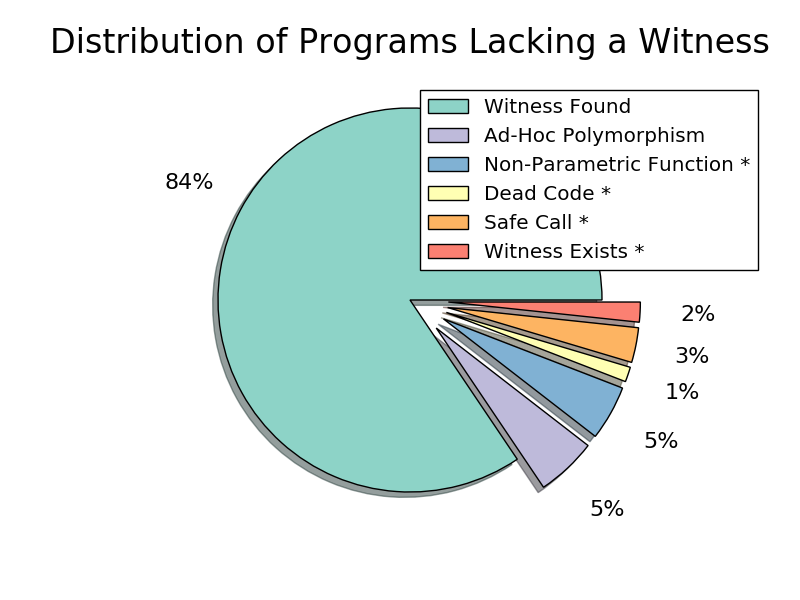
\includegraphics[width=0.7\linewidth]{nanomaly/distrib_ext.png}
\vspace{-0.75cm}
\caption{Results of our investigation into programs where \toolname
  did not produce a witness. A ``*'' denotes that the percentage is an
  estimate based on a random sampling of 50 programs.}
\label{fig:no-witness}
\end{figure}

\paragraph{Ad-Hoc Polymorphism}
%
We found that for 5\% programs \toolname got stuck when it tried to
compare two holes.
%
\ocaml provides polymorphic equality and comparison operators,
overloading them for each type.
%
While convenient to use, they pose a challenge for \toolname's
combination of execution and inference.
%
For example, consider the \hbox{@n <= 0@} test in our @fac@ example.
%
The @<=@ operator is polymorphic, but in this case we can make progress because
the literal @0@ is not.
%
Suppose, however, we parameterized @fac@ by a lower bound, \eg
%
\begin{code}
  let rec fac n m =
    if n <= m then
      true
    else
      n * fac (n - 1) m
\end{code}
%
When given @fac@, \toolname will generate two fresh holes
$\nu_1[\alpha_1]$ and $\nu_2[\alpha_2]$ and proceed directly into the
@n < m@ comparison.
%
We cannot (yet) instantiate either hole because we have no constraints
on the $\alpha$s (we know they must be equal, but nothing else), and
furthermore we do not know what constraints we may encounter later on in
the program.
%
Thus, we cannot perform the comparison and proceed, and must give up our
search for a witness, even though one obviously exists, any pair of |n|
and |m| such that |n <= m| is false.

Extending \toolname with support for symbolic execution would alleviate
this issue, as we could then begin symbolically executing the program
until we learn how to instantiate |n| and |m|.
%
Alternatively, we could \emph{speculatively} instantiate both |n| and
|m| with some arbitrary type, and proceed with execution until we
discover a type error.
%
This speculative instantiation is, of course, unsound; we would have to
take care to avoid reporting frivolous type errors that were caused by
such instantiations.
%
We would need to track which holes were instantiated speculatively 
to distinguish type errors that would have happened regardless, as
in @fac@, from type errors that were caused by our instantiation.

Further, suppose that our speculative instantiation induces a frivolous
type error.
%
For example, suppose we are given
%
\begin{code}
  let bad x y =
    if x < y then
      x *. y
    else
      0.0
\end{code}
%
and choose to (speculatively) instantiate @x@ and @y@ as @int@s and proceed
down the ``true'' branch.
%
We will quickly discover this was the wrong choice, as they are immediately
narrowed to @float@s.
%
We must now backtrack and try a different instantiation, but we no
longer need to choose one at random.
%
Since our instantiation was speculative, and @x@ and @y@
% WRW thinks "morally" is too informal for this venue. 
were \emph{originally} holes, we can treat the @*.@ operator as a normal
narrowing point with two holes.
%
This tells us that the \emph{correct} instantiation was in fact @float@,
and we can then proceed as normal from the backtracking point with a
concrete choice of @float@s.
%
Thus, it appears that speculative instantiation of holes may be a
useful, lightweight alternative to symbolic execution for our purposes.

% \paragraph{} \hspace{0ex} \\
% The remaining 473 programs for which we could not produce a witness did
% not admit such an automatic diagnosis, so we selected a random sample of
% 50 programs and manually searched for a witness.
% %
% We categorized the programs into three groups.


\paragraph{Non-Parametric Function Type *}
%
5\% of programs lack a witness in our semantics due to our
non-parametric $\tfun$ type for functions.
%
Recall that our goal is to expose the runtime errors that would have
been prevented by the type systems.
%
At runtime, it is always safe to call a function, thus we give functions
a simple type $\tfun$ that says they may be applied, but says nothing
about their inputs or outputs.
%
But consider the following @clone@ function, which is supposed to
produce a list containing @n@ copies of the input @x@.
%
% Seven programs violated the \emph{occurs check} with cyclic typing
% constraints like @'a = 'a list@, for example the following @clone@
% function.
%
\begin{code}
  let rec clone x n =
    if n > 0 then
      clone [x] (n - 1)
    else
      []
\end{code}
%
Unfortunately, the student instead constructs an @n@-level nested list
containing a single @x@.
%
The \ocaml compiler rejects this program because the recursive call to
@clone@ induces a cyclic typing constraint @'a = 'a list@, capturing the
fact that each call increases the nesting of the list.
%
\toolname fails to catch this because we do not track the types of the
inputs to @clone@.

We note, however, that @clone@ cannot go wrong; it is perfectly safe to
repeatedly enclose a list inside another (disregarding the fact that the
nested list is never returned).
%
Still, such a function would be very difficult to \emph{call} safely, as
the programmer would have to reason about the dependency between the
input @n@ and the nesting of the output list, which cannot be expressed
in \ocaml's type system.

Thus, it is not particularly satisfying that \toolname fails to produce
a witness here; a possible solution could be to track the types of the
inputs, and demonstrate to the user how they change between recursive
calls.
%
This would require maintaining a typing environment of variables in
addition to the environments we maintain for holes.
%
We would have to modify the rule $\reappgood$ from
Figure~\ref{fig:operational} to additionally $\forcesym$ the function's
type against the concrete inputs.
%
However, we would want to ensure that this $\forcesym$ cannot fail ---
it is preferable to report a stuck term as that provides a fuller view
of the error.
%
Rather, we would note which evaluation steps induced incompatible
type refinements, and if a traditional witness cannot be found, we could
then report a trace expanded to show precisely these steps.
%
This represents only a modest extension to our semantics, and would be
interesting to explore further.

\paragraph{Dead Code and ``Safe'' Function Calls *}
%
4\% of programs contained type errors that were unreachable, either
because they were dead code, or because the student called the function
with inputs that could not trigger the error.


1\% contained type errors that were unreachable by any inputs, often due
to overlapping patterns in a @match@ expression.
%
% While technically safe, dead code is generally considered a ``code
% smell''; students would likely benefit from a warning in this case.
% \ES{Wes says this is too informal, source the claim}
%
While technically safe, dead code is generally considered a maintenance
risk, as the programmer may not realize that it is dead~\cite{Wheeler2014-fg}
or may accidentally bring it back to life~\cite{Seven2014-gf}.
%
Thus, a warning like that provided by \ocaml's pattern exhaustiveness
checker would be helpful.

%\paragraph{Bad Function Calls}
A further 3\% included a function call where the
student supplied ill-typed inputs, but the path induced
by the call did not contain an error.
%
Consider the following |assoc| function, which
looks up a key in an \emph{association list}, returning a default if
it cannot be found.
%
\begin{code}
  let rec assoc (d, k, l) = match l with
    | (ki, vi)::tl ->
       if ki = k then
         vi
       else
         assoc (d, k, tl)
    | _ -> d

  let _ = assoc ([], 123, [(123, "sad"); (321, "happy")])
\end{code}
%
The student's definition of |assoc| is correct, but \ocaml rejects their
subsequent call because the default value |[]| is incompatible with the
|string| values in the list.
%
In this particular call the key |123| is in the list, so the default
will not be used (even if it were, there would not be an error) and
\ocaml's complaint is moot.
%
Of course, \ocaml cannot be expected to know that this particular call
is safe, its type system is not sophisticated enough to express the
necessary conditions.
%
% \ES{TODO: add some comment about using dependent types, though this particular example would be quite bizarre to encode in DT..}

% We note that many of the programs in this category appear to come from
% interactions with the \ocaml top-level, \ie the student defined a
% function and is now experimenting with it.
% %
% These calls are thus particularly harmless, indeed they may even be
% \emph{beneficial}, as the student may next try looking up a key that
% \emph{does not} exist, and realize that the returned values are
% incompatible.
% \ES{Wes doesn't like this, sounds like punting on the issue}

\paragraph{Witness Exists *}
%
We found that only 2\% of programs admit a witness that \toolname
was unable to discover.
%
Slightly over half involved synthesizing a \emph{pair} of
specially-crafted inputs that would result in the function returning
values of incompatible types.
%
The rest required synthesizing an input that would trigger a
particular path through the program, and would likely have been caught
by symbolic execution.

\paragraph{Summary}
%
Our investigation suggests that the vast majority of programs
for which we fail to find a witness do not, in fact, admit a
witness.
%
% Overall, it appears that our random instantiation of holes is well-suited
% to finding type errors in student programs.
These programs were generally cases where \ocaml's type system was
overly conservative.
%
Of course, the conservatism is somewhat justified as each case pointed
to code that would be difficult to use or maintain;
%
it would be interesting to investigate how demonstrate these issues in an
intuitive manner.

% \begin{enumerate}
% \item 7 infinite type. program doesn't go wrong, but could search for
%   context that would go wrong
% \item 15 monomorphic functions. recall we abstract a function's type as
%   $\tfun$ rather than $\alpha \to \beta$. (may also admit witness by
%   searching for context?)
% \item 6 dead code. type error occurs in unreachable code, ``deficiency''
%   of the type system.
% \item 14 bad call. function is well-typed, student calls makes ill-typed
%   call, but no error triggered. nothing to be done, as we do not control
%   call-site.
% \end{enumerate}

%%% Local Variables:
%%% mode: latex
%%% TeX-master: "main"
%%% End:
